\documentclass{article}
\usepackage{amsmath}
\usepackage{amssymb}
\usepackage{graphicx}
\graphicspath{{../figures/}}

\title{Low-Rank Tensor PDE Dissertation Showcase}
\author{ReproMath example}
\date{}

\begin{document}
\maketitle

\section{Project Overview}

This miniature dissertation project demonstrates how ReproMath can keep a
mathematical research workflow checkable. A low-rank tensor PDE project often
connects tensor notation, HOSVD-style approximations, numerical diagnostics,
figures, and final LaTeX writing. The purpose of this example is to keep those
artifacts small, reproducible, and mapped in \texttt{repromath.toml}.

\section{Tensor Notation}

For a third-order tensor, a mode unfolding rewrites multiway data as a matrix
view. This is not a change in the underlying data; it is a bookkeeping device
that lets matrix tools such as the singular value decomposition act on one mode
at a time.

\begin{figure}[h]
  \centering
  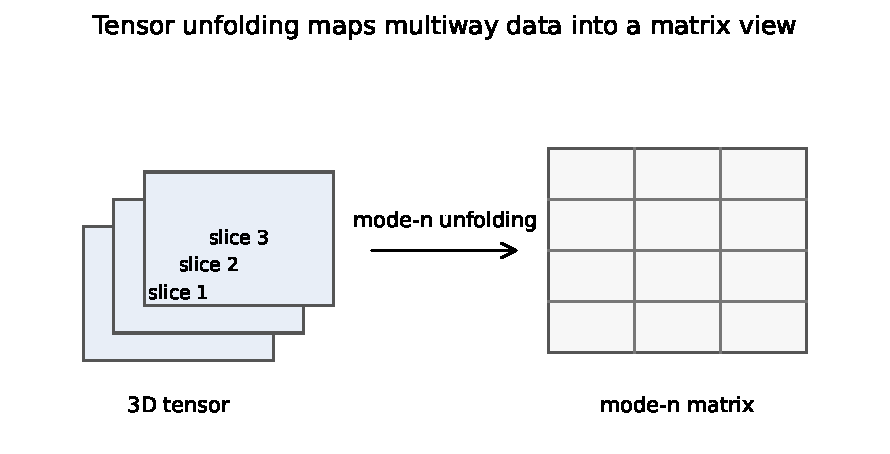
\includegraphics[width=0.78\linewidth]{tensor-unfolding.pdf}
  \caption{A conceptual mode unfolding used to connect tensor notation with
  matrix computations.}
  \label{fig:tensor-unfolding}
\end{figure}

In a truncated HOSVD study, the notebook records the factor matrices, the core
tensor, and the diagnostics needed to decide whether a chosen multilinear rank
is numerically reasonable.


\section{Numerical Diagnostics}

The first question in a low-rank approximation experiment is whether the
singular values decay quickly enough to justify truncation. Figure
\ref{fig:singular-value-decay} shows a toy comparison between fast and slow
decay.

\begin{figure}[h]
  \centering
  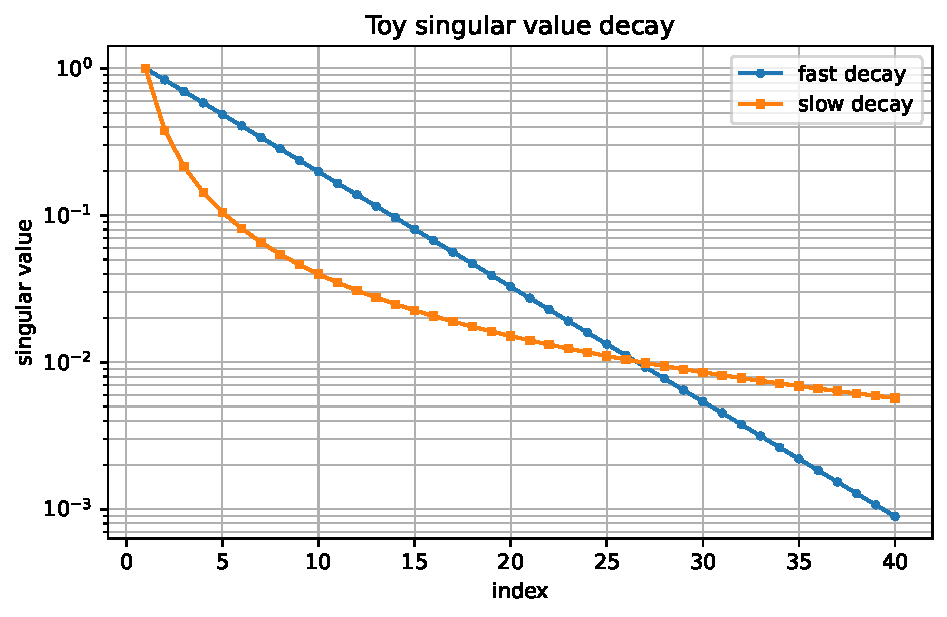
\includegraphics[width=0.72\linewidth]{singular-value-decay.pdf}
  \caption{Toy singular value decay curves used as a diagnostic for low-rank
  approximation.}
  \label{fig:singular-value-decay}
\end{figure}

The second question is whether the compressed representation saves enough
storage to justify the approximation. Figure \ref{fig:storage-vs-rank} compares
full tensor storage with a simple equal-rank Tucker storage count.

\begin{figure}[h]
  \centering
  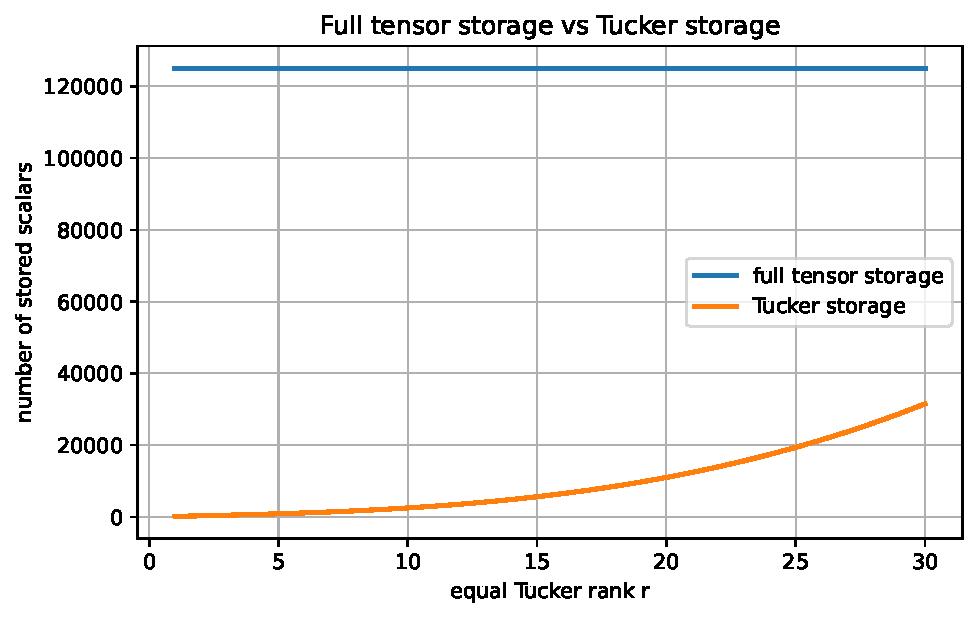
\includegraphics[width=0.72\linewidth]{storage-vs-rank.pdf}
  \caption{A lightweight storage comparison for a cubic tensor and equal Tucker
  rank.}
  \label{fig:storage-vs-rank}
\end{figure}

The corresponding notebook keeps these diagnostics close to the code that
generates them, so that dissertation figures and computational checks can be
reviewed together.



\end{document}
